\documentclass[compress,table,xcolor=dvipsnames]{beamer}\usepackage[]{graphicx}\usepackage[]{color}
%% maxwidth is the original width if it is less than linewidth
%% otherwise use linewidth (to make sure the graphics do not exceed the margin)
\makeatletter
\def\maxwidth{ %
  \ifdim\Gin@nat@width>\linewidth
    \linewidth
  \else
    \Gin@nat@width
  \fi
}
\makeatother

\definecolor{fgcolor}{rgb}{0.345, 0.345, 0.345}
\newcommand{\hlnum}[1]{\textcolor[rgb]{0.686,0.059,0.569}{#1}}%
\newcommand{\hlstr}[1]{\textcolor[rgb]{0.192,0.494,0.8}{#1}}%
\newcommand{\hlcom}[1]{\textcolor[rgb]{0.678,0.584,0.686}{\textit{#1}}}%
\newcommand{\hlopt}[1]{\textcolor[rgb]{0,0,0}{#1}}%
\newcommand{\hlstd}[1]{\textcolor[rgb]{0.345,0.345,0.345}{#1}}%
\newcommand{\hlkwa}[1]{\textcolor[rgb]{0.161,0.373,0.58}{\textbf{#1}}}%
\newcommand{\hlkwb}[1]{\textcolor[rgb]{0.69,0.353,0.396}{#1}}%
\newcommand{\hlkwc}[1]{\textcolor[rgb]{0.333,0.667,0.333}{#1}}%
\newcommand{\hlkwd}[1]{\textcolor[rgb]{0.737,0.353,0.396}{\textbf{#1}}}%

\usepackage{framed}
\makeatletter
\newenvironment{kframe}{%
 \def\at@end@of@kframe{}%
 \ifinner\ifhmode%
  \def\at@end@of@kframe{\end{minipage}}%
  \begin{minipage}{\columnwidth}%
 \fi\fi%
 \def\FrameCommand##1{\hskip\@totalleftmargin \hskip-\fboxsep
 \colorbox{shadecolor}{##1}\hskip-\fboxsep
     % There is no \\@totalrightmargin, so:
     \hskip-\linewidth \hskip-\@totalleftmargin \hskip\columnwidth}%
 \MakeFramed {\advance\hsize-\width
   \@totalleftmargin\z@ \linewidth\hsize
   \@setminipage}}%
 {\par\unskip\endMakeFramed%
 \at@end@of@kframe}
\makeatother

\definecolor{shadecolor}{rgb}{.97, .97, .97}
\definecolor{messagecolor}{rgb}{0, 0, 0}
\definecolor{warningcolor}{rgb}{1, 0, 1}
\definecolor{errorcolor}{rgb}{1, 0, 0}
\newenvironment{knitrout}{}{} % an empty environment to be redefined in TeX

\usepackage{alltt}

\usepackage{xcolor}
\usepackage{url}
\usepackage{amsmath}
\usepackage{amsthm}
\usepackage{amssymb}
\usepackage{graphicx}
\usepackage{tikz}
\usetikzlibrary{shapes,arrows}
\usepackage{float}
\usepackage{verbatim}
\usepackage{hyperref}

\usepackage{wrapfig}

\usepackage{multirow}

\usepackage{lmodern,tabularx,ragged2e,booktabs}
\newcolumntype{Y}{>{\arraybackslash\RaggedRight}X}
\newcolumntype{P}[1]{>{\arraybackslash\RaggedRight}p{#1}}

\usetheme{Szeged}
\usecolortheme[named=RoyalBlue]{structure}
\setbeamertemplate{headline}{}
\setbeamertemplate{navigation symbols}{}

% Personal Data
\def\Put(#1,#2)#3{\leavevmode\makebox(0,0){\put(#1,#2){#3}}}


\title[QC and analysis of ChIP-exo]{Data exploration, quality control
  and statistical analysis of ChIP-exo experiments}

\author{Rene Welch\\Preliminary Examination}

\institute[UW-STAT]{Department of Statistics\\University of Wisconsin - Madison}

\setbeamertemplate{section in toc}[sections numbered]
\setbeamertemplate{subsection in toc}[subsections numbered]

\setbeamertemplate{section in toc}[square]
\setbeamertemplate{subsection in toc}[square]


\date{December 1st, 2015}

\newcommand{\sig}{\sigma^{70}}
\IfFileExists{upquote.sty}{\usepackage{upquote}}{}
\begin{document}


\begin{frame}
  \maketitle
\end{frame}

\begin{frame}
\frametitle{Outline}
  \tableofcontents
\end{frame}

\section{Background}

\begin{frame}
\frametitle{ChIP-exo procedure}
  \begin{figure}[H]
    \centering
\includegraphics{../figs/diagrams/ChIPexo_diagram1.png}
\includegraphics{../figs/diagrams/ChIPexo_diagram2.png}\\
\includegraphics{../figs/diagrams/ChIPexo_diagram3.png}
    \caption{ChIP-exo procedure, Furey, 2012 \cite{chipbeyond}}
    \label{fig:exo_diagram}
  \end{figure}
\end{frame}

\section{ChIP-exo Data Exploration and Qualiy Control}

\subsection{ChIP-Seq QC measures}

\begin{frame}[t,plain]
  \frametitle{ChIP-Seq QC measures}

  \begin{itemize}
\only<1>{
  \item Number of reads. Self-explanatory, the higher the better
}
  \item<2-> Number of reads.
\only<2>{
\item PCR bottleneck Coeff. Ratio of number of pos. to which
  {\color{RoyalBlue}EXACTLY} one reads maps and number of pos. to
  which {\color{RoyalBlue}AT LEAST} one reads maps }
\only<2>{
\begin{figure}[H]
  \centering
  \includegraphics[width = .75\textwidth]{../figs/for_paper/PBC_example.pdf}
\end{figure}
}
\item<3-> PCR bottleneck Coeff.
\only<3,4>{
\item Strand Cross-Correlation. 
\begin{align}
  y(\delta) = \sum_c w_c r\left[ n_c^+ \left(x + \frac{\delta}{2}
    \right), n_c^- \left( x- \frac{\delta}{2} \right)\right]
\nonumber
\end{align}
}
\only<3>{
  \begin{figure}[H]
    \centering
    \includegraphics[width = .4\textwidth]{../figs/for_paper/Kharchenko.png}
\caption{SCC explanation. Kharchenko et al., 2008 \cite{strandcc}}
  \end{figure}
}
\only<4>{
\begin{figure}[H]
  \centering
  \includegraphics[width = \textwidth]{../figs/for_paper/SCC.png}
\caption{SCC as QC. Landt et al., 2012 \cite{encode_qc}}
\end{figure}
}
\item<5-> Strand Cross-Correlation.
\only<5>{
\item Normalized Strand Cross-Correlation. Ratio between the SCC when
  the shift is the fragment length and min. value of the SCC.
}
\end{itemize}
\end{frame}

\subsection{Evaluation of ChIP-Seq QC Metrics for ChIP-exo}
\begin{frame}[plain]
\frametitle{Evaluation of ChIP-Seq QC Metrics for ChIP-exo}

\setlength\tabcolsep{3pt}  % default value: 6pt
\scriptsize  %%  command to change the font size
% \rowcolor{RoyalBlue!20} %-- this indicates the change in odd and pair rows
\begin{table}[H]
\begin{tabularx}{\textwidth}{ @{} c|c|c|c|c|c|c| Y @{}}
  \toprule
\textbf{IP} & \textbf{Organism}  & \textbf{Condition} & \textbf{Rep.} & \textbf{Nr. reads} & \textbf{PBC} &  \textbf{NSC} & \textbf{Source} \\
\midrule
$\sig$ & E.Coli & Rif-0min & 1 & 960,256 & 0.2823 &   10.29   & \multirow{4}{\hsize}{Courtesy of Prof. Landick's lab} \\
$\sig$ &  E.Coli & Rif-0min & 2 & 2,247,295 & 0.2656 &  25.08  \\
$\sig$ &  E.Coli & Rif-20min & 1 & 1,940,387 & 0.2698 &  17.69  \\
$\sig$ &  E.Coli & Rif-20min & 2 & 4,229,574 & 0.2153 &   14.11 \\
\hline
FoxA1 &  Mouse &  - & 1 & 22,210,461 & 0.6562 & 21.452 & \multirow{3}{\hsize}{From Serandour et al., 2013 \cite{exoillumina}} \\
FoxA1 &  Mouse &  - & 2 & 22,307,557 & 0.7996 & 60.661 \\
FoxA1 &  Mouse &  - & 3 & 22,421,729 & 0.1068 & 72.312 \\
\hline
ER & Human & - & 1 & 9,289,835 & 0.8082 & 19.843 & \multirow{3}{\hsize}{From Serandour et al., 2013 \cite{exoillumina}} \\
ER & Human & - & 2 & 11,041,833 & 0.8024 & 21.422 \\
R & Human & - & 3 & 12,464,836 & 0.8203 & 19.699 \\
\hline
CTCF & Human & - & 1 &   48,478,450 & 0.4579 & 15.977 & From Rhee and Pugh 2011, \cite{exo1} \\
\bottomrule
\end{tabularx}  
\end{table}

{\small
\begin{itemize}
\item For PBC (human and mouse): 0 - 0.5 severe bottlenecking , 0.5 -
  0.8 moderate bottlenecking, 0.8 - 0.9 mild bottlenecking, 0.9 - 1 no
  bottlenecking.
\item For NSC (human and mouse): $ < 1.1$ is relatively low.
\end{itemize}
}
\end{frame}

\subsection{Comparison of ChIP-exo and ChIP-seq}


\begin{frame}
  \frametitle{Comparison of ChIP-exo and ChIP-Seq}

\begin{figure}[H]
  \centering
  \includegraphics[width = .5\textwidth,page = 3 ]{../figs/for_paper/ChIPseqPET_ChIPexo_tagCount_comparison.pdf}
  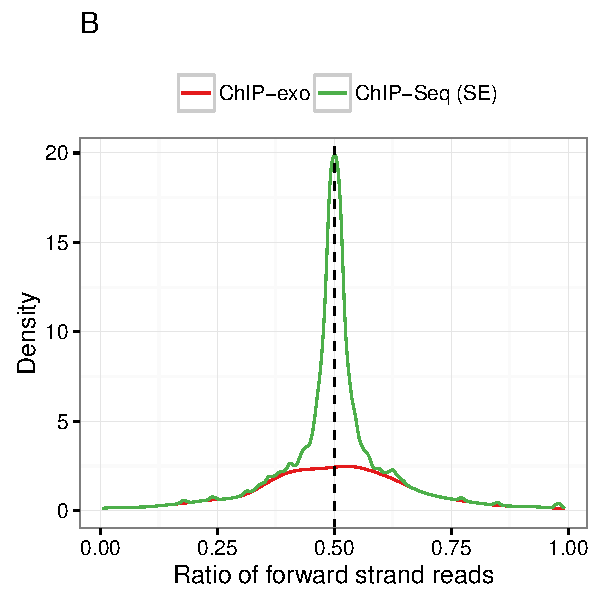
\includegraphics[width = .5\textwidth]{../figs/for_paper/forward_strand_ratio_comp_old.pdf}
\end{figure}

{\small
\begin{itemize}
\item A shows that high density regions are similar between ChIP-Seq
  and ChIP-exo but background regions are not.
\item The peak-pair assumption does hold in ChIP-exo data, but not
  locally since some regions show strand-imbalance.
\end{itemize}
}

\end{frame}

\begin{frame}[t]
  \frametitle{Comparison of ChIP-exo and ChIP-seq}  
\begin{columns}
\column{.7\textwidth}
\begin{figure}[H]
  \centering  
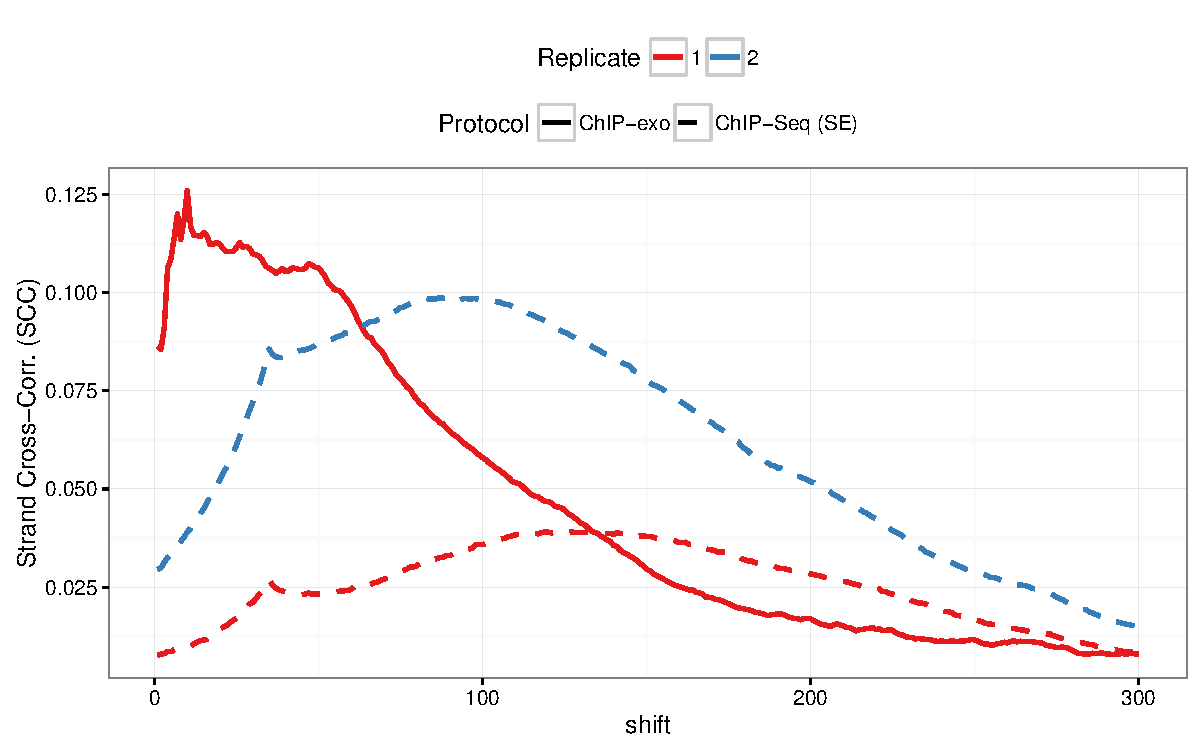
\includegraphics[width = .9\textwidth]{../figs/for_paper/scc_ctcf.pdf}
\end{figure}

\column{.3\textwidth}
  \begin{minipage}[c][.6\textheight][c]{\linewidth}
{\small
  {\color{RoyalBlue}Figure:} SCC for CTCF factor in HeLa cell line for
    ChIP-exo and SET-ChIP-Seq.\\
    - {\color{ForestGreen} PBC for rep1 is 0.56}
    - {\color{ForestGreen} PBC for rep2 is 0.94}
  }
\end{minipage}
\end{columns}

{\small
\begin{itemize}
\item There is a \emph{``phantom peak''} at read length.
\item In ChIP-Seq SCC is maximized at the unobserved fragment length.
\item In ChIP-exo, the \emph{``phantom peak''} and the fragment length
  summit are confounded.
\end{itemize}
}
\end{frame}

\subsection{Quality Control Pipeline}

\begin{frame}[t]
  \frametitle{Quality Control Pipeline}

  \begin{enumerate}
\only<1>{
  \item Partition the genome and generate ChIP-exo islands.
\begin{figure}[H]
\centering
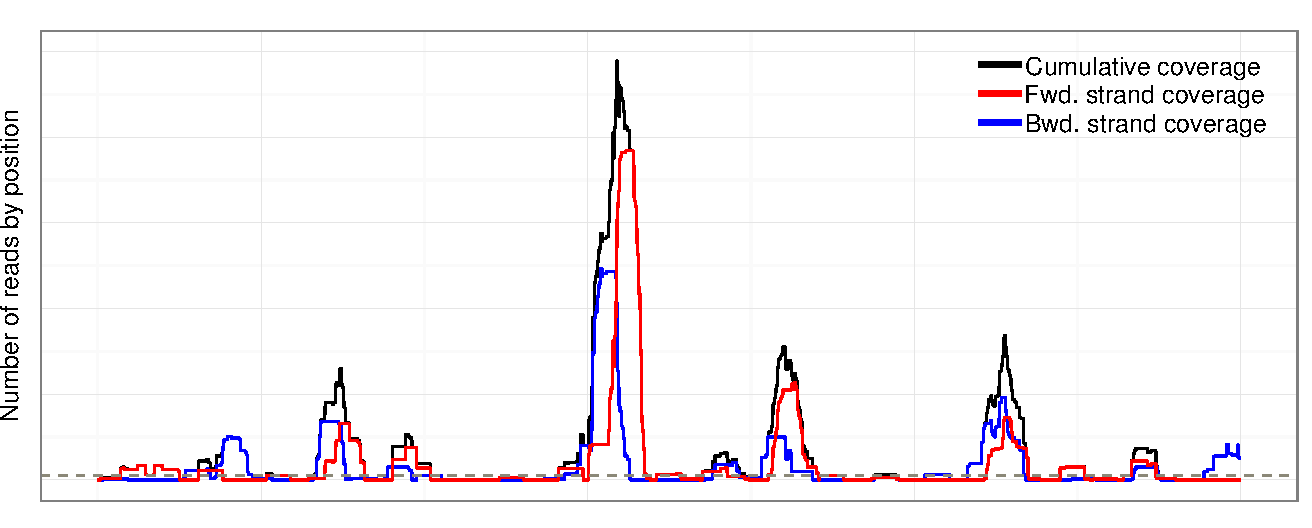
\includegraphics[width = \textwidth]{../figs/for_paper/coverage_diagram2_part1.pdf}
\end{figure}
}
\only<2>{
\addtocounter{enumi}{1}
\item Calculate a vector of summary statistics for each islands.
\begin{figure}[H]
\centering
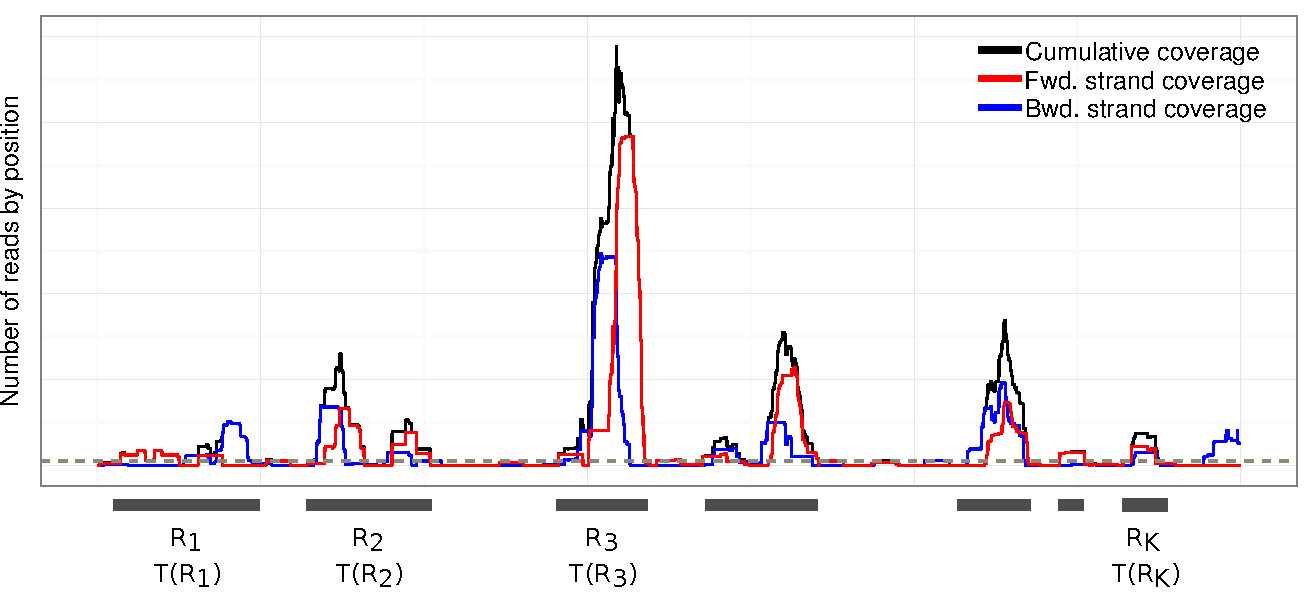
\includegraphics[width = \textwidth]{../figs/for_paper/coverage_diagram2_part2.pdf}
\end{figure}
}
\only<3>{
\addtocounter{enumi}{2}
\item Visualize all islands together.
\begin{figure}[H]
\centering
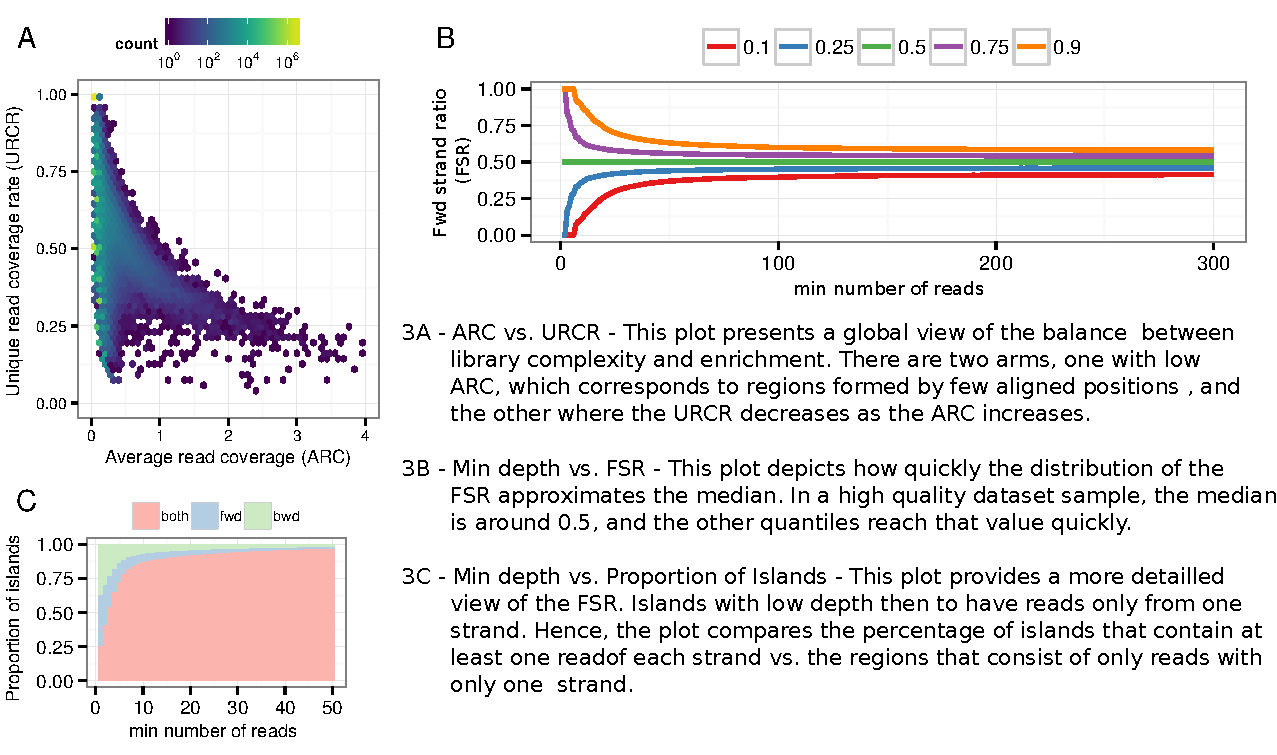
\includegraphics[width = \textwidth]{../figs/for_paper/coverage_diagram2_part3P.pdf}
\end{figure}
}
  \end{enumerate}
\end{frame}


 % \begin{itemize}
  % \item $\mbox{local-NSC}$
  % \item $\mbox{FSR} = \frac{\text{Nr. of fwd. strand reads in region}}{\text{Nr. of reads in region}}$
  % \end{itemize}  


\begin{frame}
  \frametitle{ARC vs. URCR exploration}
\only<1>{
  \begin{itemize}
  \item $\mbox{ARC} = \frac{\text{Nr. of reads in the
        region}}{\text{Width of the region}}$
  \item $\mbox{URCR} = \frac{\text{Nr. of reads mapped to only one
        position in the region}}{\text{Nr. of reads in the region}}$
  \end{itemize}
}
\only<2>{
All regions
  \begin{figure}[H]
    \centering
    \includegraphics[width = .7\textwidth,page = 1]{../figs/for_paper/ARC_vs_URCR_example_npos.pdf}
  \end{figure}
}

\only<3>{
Mapped to more than 10 positions
  \begin{figure}[H]
    \centering
    \includegraphics[width = .7\textwidth,page = 2]{../figs/for_paper/ARC_vs_URCR_example_npos.pdf}
  \end{figure}
}

\only<4>{
Mapped to more than 30 positions
  \begin{figure}[H]
    \centering
    \includegraphics[width = .7\textwidth,page = 3]{../figs/for_paper/ARC_vs_URCR_example_npos.pdf}
  \end{figure}
}
\only<5>{
Mapped to more than 50 positions
  \begin{figure}[H]
    \centering
    \includegraphics[width = .7\textwidth,page = 4]{../figs/for_paper/ARC_vs_URCR_example_npos.pdf}
  \end{figure}
}

\end{frame}


\begin{frame}
  \frametitle{ARC vs. URCR exploration}

\only<1-2>{
  \begin{figure}[H]
    \centering
    \includegraphics[width = .7\textwidth,page =1]{../figs/for_paper/enrichment_example.pdf}
  \end{figure}
}

\only<2>{
\Put(120,200){\includegraphics[width = .6\textwidth,page = 1]{../figs/for_paper/coverage_example.pdf}}
}

\only<3-4>{
  \begin{figure}[H]
    \centering
    \includegraphics[width = .7\textwidth,page =2]{../figs/for_paper/enrichment_example.pdf}
  \end{figure}
}

\only<4>{
\Put(120,200){\includegraphics[width = .6\textwidth,page = 2]{../figs/for_paper/coverage_example.pdf}}
}

\only<5-6>{
  \begin{figure}[H]
    \centering
    \includegraphics[width = .7\textwidth,page =3]{../figs/for_paper/enrichment_example.pdf}
  \end{figure}
}

\only<6>{
\Put(120,200){\includegraphics[width = .6\textwidth,page = 3]{../figs/for_paper/coverage_example.pdf}}
}

\only<7-8>{
  \begin{figure}[H]
    \centering
    \includegraphics[width = .7\textwidth,page = 4]{../figs/for_paper/enrichment_example.pdf}
  \end{figure}
}

\only<8>{
\Put(120,200){\includegraphics[width = .6\textwidth,page = 4]{../figs/for_paper/coverage_example.pdf}}
}

% \only<9-10>{
%   \begin{figure}[H]
%     \centering
%     \includegraphics[width = .7\textwidth,page = 5]{../figs/for_paper/enrichment_example.pdf}
%   \end{figure}
% }

% \only<10>{
% \Put(120,200){\includegraphics[width = .6\textwidth,page = 5]{../figs/for_paper/coverage_example.pdf}}
% }

\only<9-10>{
  \begin{figure}[H]
    \centering
    \includegraphics[width = .7\textwidth,page =6]{../figs/for_paper/enrichment_example.pdf}
  \end{figure}
}

\only<10>{
\Put(120,300){\includegraphics[width = .6\textwidth,page = 6]{../figs/for_paper/coverage_example.pdf}}
}

\only<11-12>{
  \begin{figure}[H]
    \centering
    \includegraphics[width = .7\textwidth,page =7]{../figs/for_paper/enrichment_example.pdf}
  \end{figure}
}

\only<12>{
\Put(120,300){\includegraphics[width = .6\textwidth,page = 7]{../figs/for_paper/coverage_example.pdf}}
}

\only<13-14>{
  \begin{figure}[H]
    \centering
    \includegraphics[width = .7\textwidth,page =8]{../figs/for_paper/enrichment_example.pdf}
  \end{figure}
}

\only<14>{
\Put(120,300){\includegraphics[width = .6\textwidth,page = 8]{../figs/for_paper/coverage_example.pdf}}
}


\end{frame}

\begin{frame}
  \frametitle{ARC vs. URCR exploration by replicate}
\only<1>{
All regions
\begin{figure}[H]
  \centering
  \includegraphics[width = \textwidth,page = 1]{../figs/Carroll_mice_for_paper/FoxA1_enrichment.pdf}
\end{figure}
}

\only<2>{
Regions formed by reads aligned to more than 10 unique positions
\begin{figure}[H]
  \centering
  \includegraphics[width = \textwidth,page = 3]{../figs/Carroll_mice_for_paper/FoxA1_enrichment.pdf}
\end{figure}
}

\only<3>{
Regions formed by reads aligned to more than 30 unique positions
\begin{figure}[H]
  \centering
  \includegraphics[width = \textwidth,page = 4]{../figs/Carroll_mice_for_paper/FoxA1_enrichment.pdf}
\end{figure}
}


\end{frame}


\begin{frame}
  \frametitle{ARC vs. URCR and local-NSC}

\only<1>{
Calculate coverage for all regions
\begin{figure}[H]
  \centering
  \includegraphics[width = \textwidth,page = 1]{../figs/for_paper/local_SCC_separated.pdf}
\end{figure}
}

\only<2>{
Calculate $\mbox{local-SCC}$ for regions
\begin{figure}[H]
  \centering
  \includegraphics[width = \textwidth,page = 2]{../figs/for_paper/local_SCC_separated.pdf}
\end{figure}
}

\only<3>{
Fit local polynomial regression for the $\mbox{local-SCC}$ 
\begin{figure}[H]
  \centering
  \includegraphics[width = \textwidth,page = 3]{../figs/for_paper/local_SCC_separated.pdf}
\end{figure}
}



\only<4>{
\begin{align}
 y(\delta) = f(x_\delta) + \epsilon_\delta, \quad 
\mbox{local-NSC} = \frac{max_{x_\delta} \hat{f}(x_\delta)}{\hat{\sigma}_f},
\nonumber
\end{align}
\vspace*{\fill}
}

\only<4>{
\begin{columns}

\column{.4\textwidth}
where:

\begin{itemize}
\item $x_\delta$ is the shift.
\item $y_\delta$ is the local - SCC at shift $x_\delta$
\item $\epsilon \sim N(0, \sigma^2)$ i.i.d 
\end{itemize}


\column{.6\textwidth}
{\scriptsize
  \begin{table}[H]
    \centering
    \begin{tabularx}{\textwidth}{ @{} l | r | r |r @{}}
      \toprule
      Replicate & $\hat{\sigma}$ & $\max_{x_\delta} \hat{f}(x_\delta)$ & $\mbox{local-NSC}$ \\
      \midrule
Rep. 1 & 0.0533 & 0.2215 & 4.14 \\
Rep. 2 & 0.0453 & 0.1606 & 3.54 \\
Rep. 3 & 0.0475 & 0.0832 & 1.75 \\
\bottomrule
    \end{tabularx}
  \end{table}
}

\end{columns}
}

\only<5>{
  \begin{figure}[H]
    \centering
      \includegraphics[width = \textwidth,page =4]{../figs/Carroll_mice_for_paper/Local_SCC_indicator_by_strata.pdf}
  \end{figure}

  \begin{itemize}
  \item {\color{RoyalBlue} high:} Number of unique positions $ > 100$
  \item {\color{RoyalBlue} med:} Number of unique positions in $(50,100)$
  \item {\color{RoyalBlue} low:} Number of unique positions in $(20,50)$
  \end{itemize}
}
\end{frame}



\begin{frame}[t]
  \frametitle{Strand imbalance}

\begin{figure}[H]
  \centering  
  \includegraphics[width = \textwidth,page = 3]{../figs/Carroll_mice_for_paper/Strand_imbalance.pdf} 
  \label{fig:strand}
\end{figure}

{\scriptsize
\begin{itemize}
\item 
\end{itemize}
}



\end{frame}

\section{Systematic Evaluation of ChIP-Seq and ChIP-exo}


\begin{frame}[plain]
  \frametitle{dPeak model for SET case}

\only<1>{

      \begin{figure}[H]
        \centering
        \includegraphics[width =
        \textwidth]{/p/keles/ChIPexo/volume3/ChIPexo/poster/dpeak.png}
      \end{figure}
}

\only<2>{
\begin{columns}[t]
\column{.3\textwidth}
  \begin{figure}[H]
    \centering
    \includegraphics[width =\textwidth]
{/p/keles/ChIPexo/volume3/ChIPexo/poster/dpeak.png}
  \end{figure}
  
\column{.7\textwidth}
  We consider a region with $n$ reads and $m$ positions, for the
  $i$-th read:
  \begin{itemize}
  \item $Z_i \sim \mbox{Multi}(\pi_0,\pi_1,\cdots,\pi_{g^*})$
  \item $D_i \sim \mbox{Ber}(p_D)$
    \begin{itemize}
    \item The read is in the forward strand ($D_i = 1$):
      \begin{itemize}
      \item The reads belongs to the background: $R_i | Z_i = 0, D_i =
        1 \sim \mbox{Unif}(1, m)$
      \item The read belong to the $g$-th binding event: $R_i | Z_i =
        g, D_i = 1 \sim \mbox{N}(\mu_g - \delta , \sigma^2)$
      \end{itemize}
    \item The read is in the backward strand ($D_i = 0$):
      \begin{itemize}
      \item The reads belongs to the background: $R_i | Z_i = 0, D_i =
        0 \sim \mbox{Unif}(1 , m )$
      \item The read belong to the $g$-th binding event: $R_i | Z_i =
        g, D_i = 0 \sim \mbox{N}(\mu_g + \delta , \sigma^2)$
      \end{itemize}
    \end{itemize}
  \end{itemize}
\end{columns}
}


\end{frame}


\begin{frame}[plain]
  \frametitle{Data structure}
Data available for $\sig$:
  \begin{figure}[H]
    \centering
    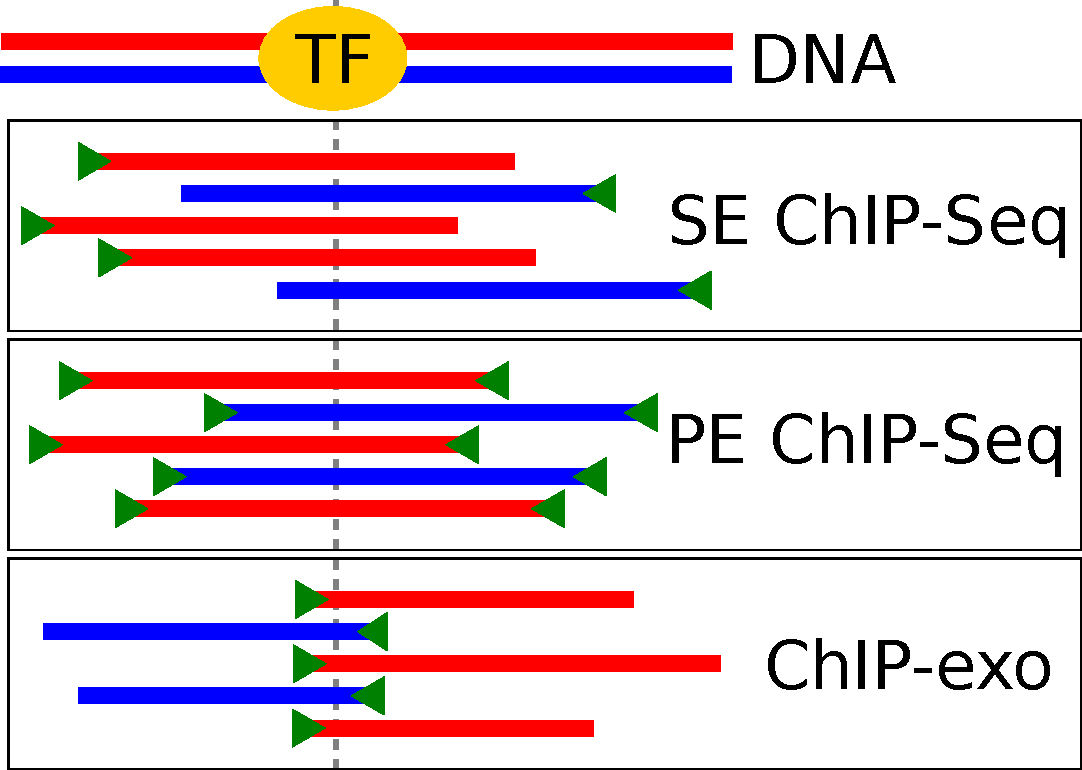
\includegraphics[width = \textwidth]{../figs/for_paper/chip_explanation.pdf}
  \end{figure}
  

\end{frame}

\begin{frame}
\frametitle{Comparison with ChIP-Seq using dPeak}
\only<1>{
  \begin{figure}[H]
  \centering
  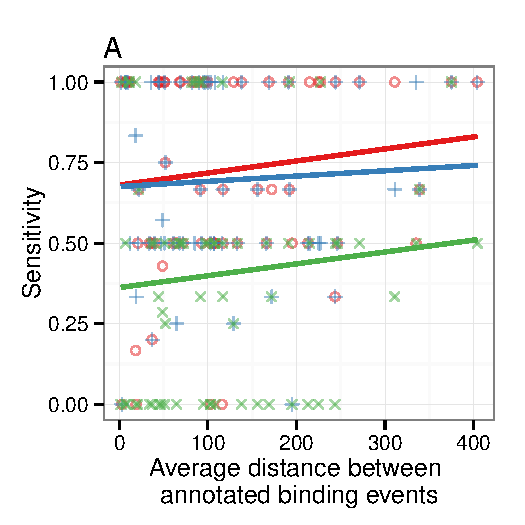
\includegraphics[width = .46\textwidth]{../figs/for_paper/sensitivity_exo_olda_data.pdf}
  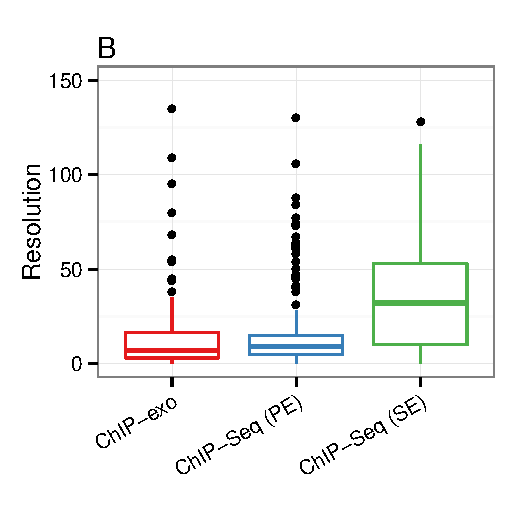
\includegraphics[width = .46\textwidth]{../figs/for_paper/resolution_by_dataset_old_data.pdf}
\end{figure}
}
\only<1>{
{\small
  \begin{itemize}
  \item Sensitivity is the defined as the proportion of identified
    peaks (regulonDB \cite{regulonDB} is used as gold-standard)
  \item Resolution is defined as the min. absolute distance of a
    regulonDB annotation to an est. binding location.
  \end{itemize}
}}

\only<2>{
\begin{figure}[H]
\centering
   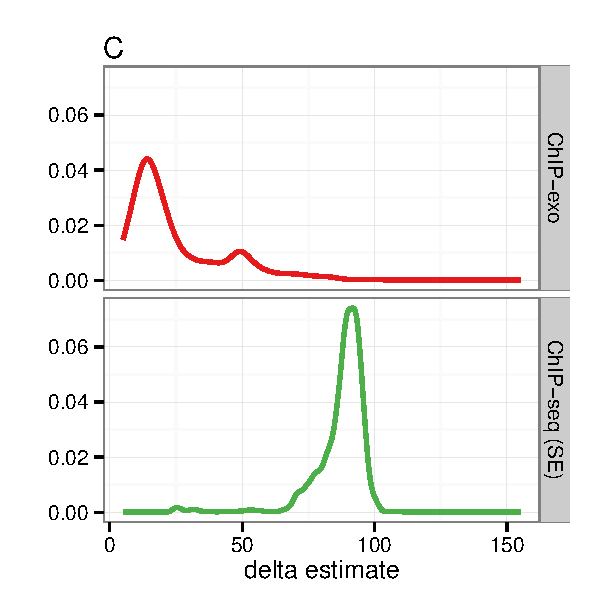
\includegraphics[width = .46\textwidth,page = 1]{../figs/for_paper/sigma_delta_old_densities.pdf}
   \includegraphics[width = .46\textwidth,page = 2]{../figs/for_paper/sigma_delta_old_densities.pdf} 
 \end{figure}
}
\only<2>{
{\small
\begin{itemize}
\item $\delta$ measures the average distance of reads to their
  respective binding sites.
\item $\sigma$ measures the dispersion of reads around their
  respective binding sites.
\item Good news !! the model is reflecting the truth.
\end{itemize}
}}
\end{frame}

\begin{frame}[t]
  \frametitle{ChIP-Seq comparison at fixed depth}

  We sampled $n$ fragment reads of each dataset ($2n$ for PET
  ChIP-Seq), and applied the MOSAiCS / dPeak pipeline:

\only<1>{
\begin{figure}[H]
  \centering
  \includegraphics[width = .4\textwidth,page = 1]{../figs/for_paper/saturation_analysis_old_frames.pdf}
  \includegraphics[width = .4\textwidth,page = 2]{../figs/for_paper/saturation_analysis_old_frames.pdf}
\end{figure}
}

\only<2>{
\begin{figure}[H]
\centering
\includegraphics[width = .4\textwidth,page = 3]{../figs/for_paper/saturation_analysis_old_frames.pdf}
  \includegraphics[width = .4\textwidth,page = 4]{../figs/for_paper/saturation_analysis_old_frames.pdf}
\end{figure}
}

\only<2>{
{\small
  \begin{itemize}
  \item ChIP-exo and PET ChIP-Seq are comparable and outperform SET
    ChIP-Seq
  \end{itemize}
}}


\end{frame}

\section{Comparison with Other Algorithms}
\begin{frame}
\frametitle{Comparison with Other Algorithms}

\begin{figure}[H]
  \centering
  \includegraphics[width = .7\textwidth]{../figs/for_paper/algorithm_resolution.pdf}
\end{figure}
  
\end{frame}

\section{Conclusions and future work}

\begin{frame}
  \frametitle{Conclusions}

  \begin{itemize}
  \item Our pipeline is capable of assessing the balance between
    sample enrichment and library complexity.
  \item We shown that the ``peak-pair'' assumption doesn't hold well
    in practice, and implemented a visualization capable of detecting
    strand imbalance.
  \item We updated dPeak, which makes a striking balance in
    sensitivity, specificity and spatial resolution.
  \item ChIP-exo and PET ChIP-Seq are comparable in resolution and
    sensitivity, and both outperform SET ChIP-Seq.
  \item We showed that with a fixed number of reads, ChIP-exo
    outperforms PET and SET ChIP-Seq.
  \item dPeak outperforms other algorithms in resolution.
  \end{itemize}
\end{frame}


\begin{frame}
\frametitle{Future work}  

\begin{itemize}
\item In the paper, we showed that there is a relationship between
  ChIP-exo tag counts and both mappability and GC content scores. We
  want to add a QC measure to the pipeline based on them.
\item We want to assess if ChIP-Nexus library complexity is actually
  higher than ChIP-exo's by using the $\mbox{local-NSC}$.
\item We have been studying E. Coli's transcription initiation
  complexes with PET ChIP-Seq. We want to improve this analysis by
  using ChIP-exo data.
\item Find a optimal strategy for labeling enhancer out of a
  predetermined list of regions in the genome by the use of active
  learning techniques.
\end{itemize}

\end{frame}

\begin{frame}[t]
\frametitle{Software}  
\begin{itemize}
\item {\color{RoyalBlue}\textbf{dPeak}}: We updated the initialization
  strategy. The latest version is currently available from
  \url{http://dongjunchung.github.io/dpeak/}.
\item {\color{RoyalBlue}\textbf{ChIPexoQual}}: This package contains
  the QC pipeline for ChIP-exo. The last version is available in
  \url{https://github.com/welch16/ChIPexoQual}.
\item {\color{RoyalBlue}\textbf{Segvis}}: The goal of this package is
  to visualize genomic regions by using aligned reads. The latest
  version is available in \url{https://github.com/keleslab/Segvis}.
\item {\color{RoyalBlue}\textbf{ChIPUtils}}: This package attempts to
  gather the most commonly used ChIP-Seq QC.The latest available
  version is in \url{https://github.com/welch16/ChIPUtils}.
\end{itemize}

\end{frame}

\begin{frame}[plain]
  
{\Huge
{\color{RoyalBlue}
\begin{center}
  \textbf{Thank you very much!}
\end{center}
}
}


\end{frame}


\begin{frame}[allowframebreaks]
  \frametitle{References}

{\tiny

\nocite{exo1}
\nocite{dpeak}

\bibliographystyle{plain} % Style BST file (bmc-mathphys, vancouver, spbasic)
\bibliography{chip_exo_paper}

}

\end{frame}

\end{document}

% LocalWords:  regulonDoB
